\section{Condition scores and paired effects}
All 300 inputs were scored successfully. Table~\ref{tab:means} and Figure~\ref{fig:means} show the mean scores for each condition. Mean scores follow $B>A>N$ for correct steps and $A>N>B$ for incorrect steps. Compared with N, A raises the mean score for both target types. Compared with B, however, A has a lower mean score for correct steps and a higher mean score for incorrect steps.

\begin{table}[!htbp]
\centering\small
\caption{Mean target scores and correct--incorrect gaps over 50 questions. B, N, and A denote baseline, neutral, and confident wording.}
\label{tab:means}
\begin{tabular}{lrrr}\toprule
 & B & N & A\\\midrule
Correct & 0.7398 & 0.7102 & 0.7267 \\
Incorrect & 0.2699 & 0.2791 & 0.2934 \\
Correct $-$ incorrect & 0.4699 & 0.4311 & 0.4333 \\
\bottomrule\end{tabular}

\end{table}

\begin{figure}[!htbp]
\centering
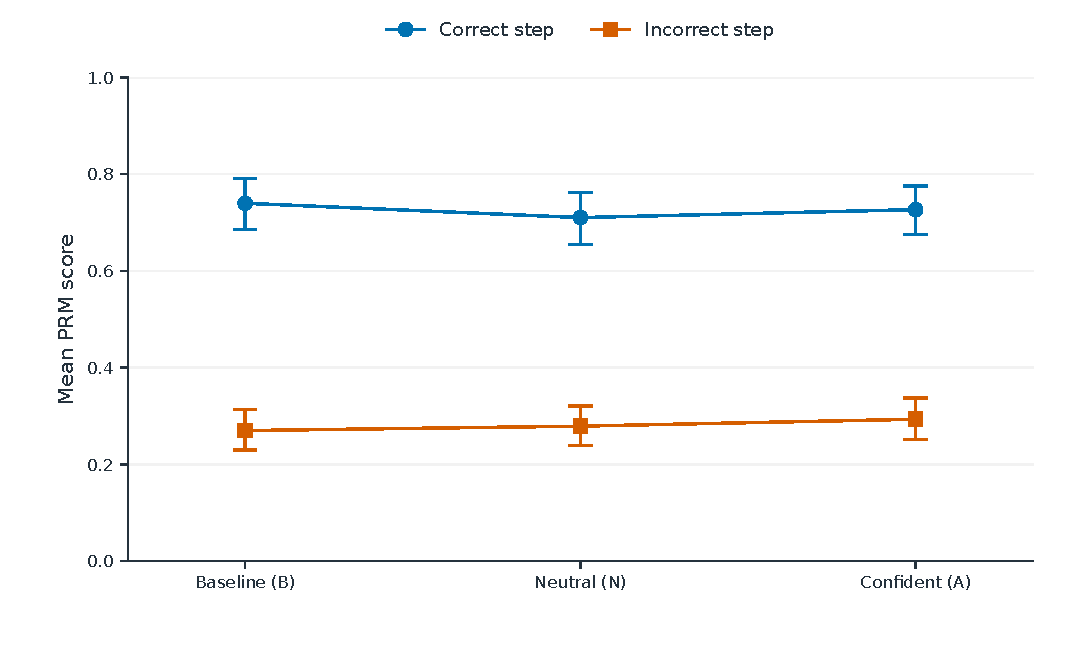
\includegraphics[width=.82\textwidth]{images/figure_1_condition_scores.pdf}
\caption{Mean target scores with pointwise 95\% bootstrap intervals. Differences are assessed using paired contrasts, rather than overlap between these marginal intervals.}
\label{fig:means}
\end{figure}

The mean incorrect-step effect is \WrongMean{} (Table~\ref{tab:effects}). The 95\% bootstrap interval includes zero, so the data do not provide clear evidence of a positive mean effect for the tested phrase replacement.

\begin{table}[!htbp]
\centering\small
\caption{Paired wording contrasts. Intervals are pointwise 95\% percentile bootstrap intervals, without multiplicity correction.}
\label{tab:effects}
\begin{tabular}{lrr}\toprule
Contrast & Mean & 95\% interval\\\midrule
Incorrect-step effect $\overline{\delta}_E$ & \WrongMean{} & \WrongCI{} \\
Correct-step effect $\overline{\delta}_C$ & \CorrectMean{} & \CorrectCI{} \\
Gap reduction $\overline{r}$ & \ReductionMean{} & \ReductionCI{} \\
\bottomrule\end{tabular}

\end{table}

Figure~\ref{fig:individual} shows the incorrect-step effects for all 50 questions. Scores rise in 29 questions and fall in 21. The median effect is $+0.0090$, and effects range from $-0.1786$ to $+0.1895$. The largest changes in either direction are much larger than the mean shift, and positive and negative changes partly cancel when averaged. The increasing profile follows from sorting by effect size; it does not indicate a trend with question difficulty or original question number.

\begin{figure}[!tbp]
\centering
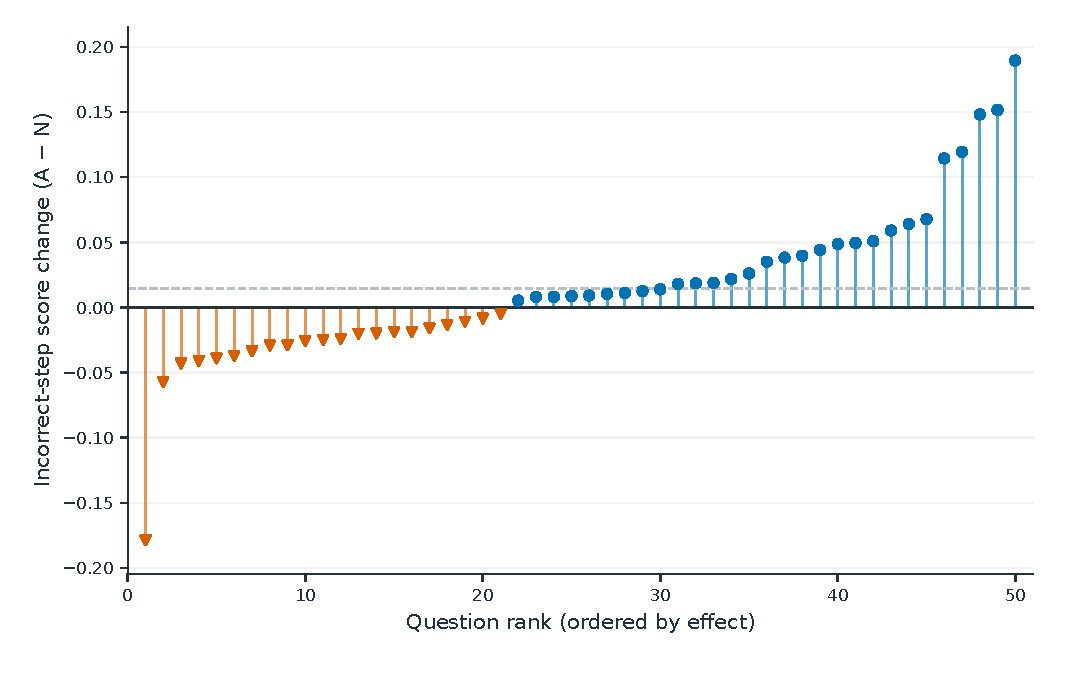
\includegraphics[width=.82\textwidth]{images/figure_2_question_effects.pdf}
\caption{Incorrect-step effects ($E$--$A$ minus $E$--$N$) for all 50 questions, sorted by effect. Each point is one question; the dashed line marks the mean.}
\label{fig:individual}
\end{figure}

Correct-step scores rise by \CorrectMean{} on average, with an interval above zero. The two mean increases are similar in size, so the mean gap changes little: it is 0.4311 under neutral wording and 0.4333 under confident wording. The gap reduction is \ReductionMean{}, with interval \ReductionCI{}. Figure~\ref{fig:gaps} displays the paired gaps and the three contrasts. The point estimate suggests slightly wider separation under confident wording, but its interval allows changes in either direction.

In the left panel of Figure~\ref{fig:gaps}, 20 points lie below the equality line, indicating a smaller gap under A, while 30 lie above it, indicating a wider gap. Correct targets still outscore their paired incorrect targets for all 50 questions under B, N, and A, with no ties.

\begin{figure}[!htbp]
\centering
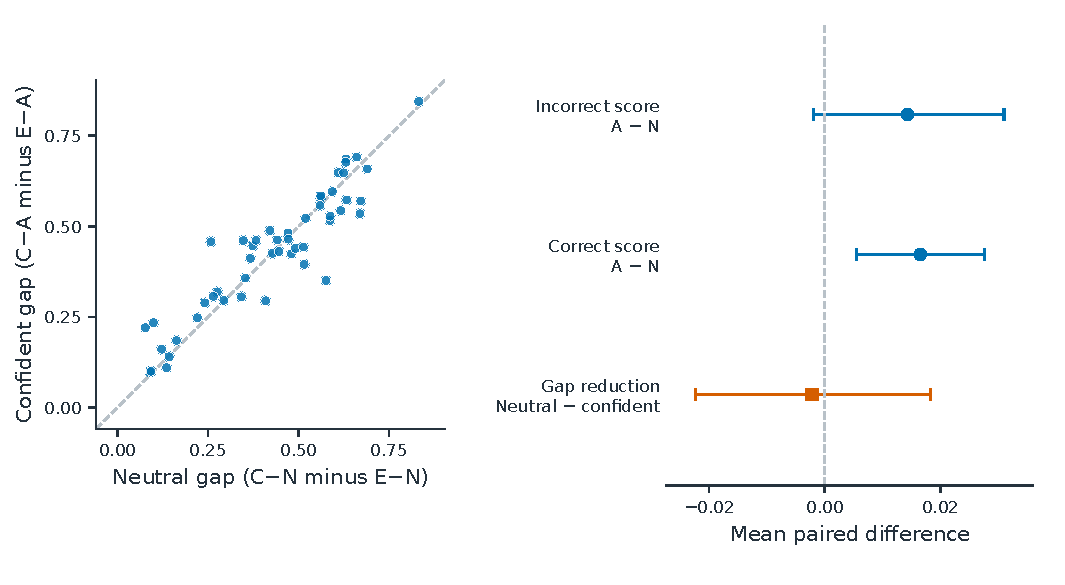
\includegraphics[width=.92\textwidth]{images/figure_3_gap_robustness.pdf}
\caption{Left: correct--incorrect gaps for each question under N and A; the diagonal marks equality. Right: mean paired effects with pointwise 95\% bootstrap intervals. Positive gap reduction means narrower separation under A.}
\label{fig:gaps}
\end{figure}

\section{Exploratory baseline comparisons}
Post hoc checks during the project audit compare both added phrases with the unprefixed baseline. These exploratory comparisons are separate from the primary comparison between A and N. Their intervals are not adjusted for multiple comparisons. The mean gap under B is 0.4699. Compared with B, the mean gap decreases by 0.0388 under N (95\% interval: $[0.0230, 0.0545]$) and by 0.0366 under A (95\% interval: $[0.0203, 0.0540]$).

Table~\ref{tab:baseline} shows the changes in correct- and incorrect-step scores separately. Compared with B, both N and A have lower mean correct-step scores and higher mean incorrect-step scores. Both changes contribute to the smaller gap: the reduction equals the incorrect-step score change minus the correct-step score change. The intervals reported above apply only to the gap reductions.

\begin{table}[!htbp]
\centering\small
\caption{Post hoc changes relative to B, averaged over 50 questions. Score changes are N or A minus B; gap reductions are B minus N or A. Each value is computed before rounding.}
\label{tab:baseline}
\begin{tabular}{lrrr}
\toprule
Comparison & Correct-step change & Incorrect-step change & Gap reduction \\
\midrule
N versus B & $-0.0297$ & $+0.0092$ & $+0.0388$ \\
A versus B & $-0.0131$ & $+0.0235$ & $+0.0366$ \\
\bottomrule
\end{tabular}

\end{table}
